\documentclass[tikz, border = 2mm]{standalone}
\usepackage{pgfplots}

\pgfkeys{/pgfplots/Delta Style/.style={
    % scale only axis,
    % grid=major,
    axis equal,
    grid style={dashed, gray!30}, %Uncomment these lines for no grid
    axis lines=middle,
    inner axis line style={=stealth}, %Arrow type
    ultra thick,
    xlabel={\large $x$},
    ylabel={\large $y$},
    cycle list = {black,black!70,black!40,black!10} %Plot colors cycle in grayscale
  }}


\pgfplotsset{compat=1.10}
\usepgfplotslibrary{fillbetween}
\usetikzlibrary{patterns}

\usetikzlibrary{shapes}

\tikzset{My Arrow Style/.style={single arrow, fill=blue!25, anchor=base, align=center,text width=1cm}}
\newcommand{\MyArrow}[2][]{\tikz[baseline] \node [My Arrow Style,#1] {#2};}


\begin{document}
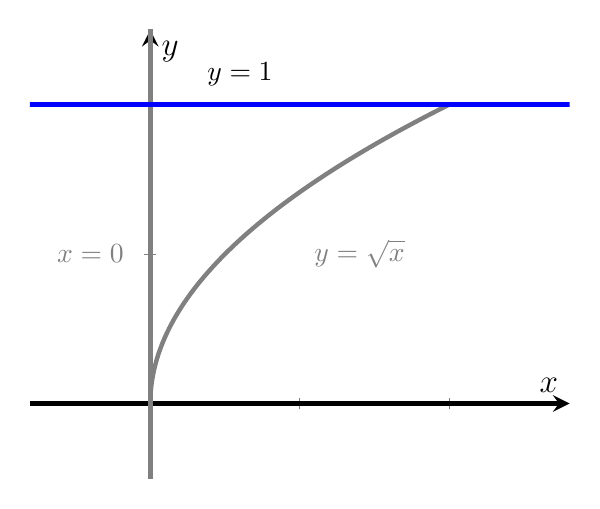
\begin{tikzpicture}
  \begin{axis} [
    Delta Style,
    xmin = -0.25,
    xmax = 1.25,
    ymin = -0.25,
    ymax = 1.25,
    xticklabels = {$ $,$ $,$ $,$ $,$ $,$ $,$ $,$ $,$ $},
    yticklabels = {$ $,$ $,$ $,$ $,$ $,$ $,$ $,$ $,$ $}
    ]

    % \addplot[name path=f,domain = 0:1,ultra thin, opacity=1, opacity = 0] {1};

    % \addplot[name path=axis, domain = 0:1, ultra thin, opacity=0] ({x^2},{x});

    % \addplot [
    %     thick,
    %     color=black,
    %     fill=black,
    %     fill opacity=0.10
    % ]
    % fill between[
    %     of=f and axis,
    %     soft clip={domain=0:1},
    % ];
    
    \addplot [mark=none,ultra thick, gray, samples=200, domain=0:1] ({x^2}, {x});
    \addplot [mark=none,  ultra thick, gray] (0,x);
    \addplot [mark=none, ultra thick, blue] (x,1);
    % \addplot [mark=none, dotted, ultra thick, gray] (x,0);
    
    \node[gray] at (axis cs:-0.2,0.5){$x=0$};
    \node[gray] at (axis cs: 0.7,0.5){$y = \sqrt{x}$};
    % \node[] at (axis cs: 0.3,-0.1){$y=0$};
    \node[] at (axis cs: 0.3,1.1){$y=1$};

  \end{axis}
\end{tikzpicture}
\end{document}